\documentclass{article}

\usepackage{fancyhdr}
\usepackage{extramarks}
\usepackage{amsmath}
\usepackage{amsthm}
\usepackage{amsfonts}
\usepackage{tikz}
\usepackage[plain]{algorithm}
\usepackage{algpseudocode}
\usepackage{amssymb}

\usetikzlibrary{automata,positioning}

%
% Basic Document Settings
%

\topmargin=-0.45in
\evensidemargin=0in
\oddsidemargin=0in
\textwidth=6.5in
\textheight=9.0in
\headsep=0.25in

\linespread{1.1}

\pagestyle{fancy}
\lhead{\hmwkAuthorName}
\chead{\hmwkClass\ (\hmwkClassInstructor\ \hmwkClassTime): \hmwkTitle}
\rhead{\firstxmark}
\lfoot{\lastxmark}
\cfoot{\thepage}

\renewcommand\headrulewidth{0.4pt}
\renewcommand\footrulewidth{0.4pt}

\setlength\parindent{0pt}

%
% Create Problem Sections
%

\newcommand{\enterProblemHeader}[1]{
    \nobreak\extramarks{}{Problem \arabic{#1} continued on next page\ldots}\nobreak{}
    \nobreak\extramarks{Problem \arabic{#1} (continued)}{Problem \arabic{#1} continued on next page\ldots}\nobreak{}
}

\newcommand{\exitProblemHeader}[1]{
    \nobreak\extramarks{Problem \arabic{#1} (continued)}{Problem \arabic{#1} continued on next page\ldots}\nobreak{}
    \stepcounter{#1}
    \nobreak\extramarks{Problem \arabic{#1}}{}\nobreak{}
}

\setcounter{secnumdepth}{0}
\newcounter{partCounter}
\newcounter{homeworkProblemCounter}
\setcounter{homeworkProblemCounter}{1}
\nobreak\extramarks{Problem \arabic{homeworkProblemCounter}}{}\nobreak{}

%
% Homework Problem Environment
%
% This environment takes an optional argument. When given, it will adjust the
% problem counter. This is useful for when the problems given for your
% assignment aren't sequential. See the last 3 problems of this template for an
% example.
%
\newenvironment{homeworkProblem}[1][-1]{
    \ifnum#1>0
        \setcounter{homeworkProblemCounter}{#1}
    \fi
    \section{Problem \arabic{homeworkProblemCounter}}
    \setcounter{partCounter}{1}
    \enterProblemHeader{homeworkProblemCounter}
}{
    \exitProblemHeader{homeworkProblemCounter}
}

%
% Homework Details
%   - Title
%   - Due date
%   - Class
%   - Section/Time
%   - Instructor
%   - Author
%

\newcommand{\hmwkTitle}{Homework\ \#2}
\newcommand{\hmwkDueDate}{October 23, 2017}
\newcommand{\hmwkClass}{Convex Optimization}
%\newcommand{\hmwkClassTime}{Section A}
\newcommand{\hmwkClassInstructor}{Professor Ying Cui}
%\newcommand{\hmwkAuthorName}{\textbf{Josh Davis} \and \textbf{Davis Josh}}
\newcommand{\hmwkAuthorName}{\textbf{Xiaoyi He}}

%
% Title Page
%

\title{
    \vspace{2in}
    \textmd{\textbf{\hmwkClass:\ \hmwkTitle}}\\
    \normalsize\vspace{0.1in}\small{Due\ on\ \hmwkDueDate\ at 11:59pm}\\
    \vspace{0.1in}\large{\textit{\hmwkClassInstructor\ \hmwkClassTime}}
    \vspace{3in}
}

\author{\hmwkAuthorName}
\date{}

%\renewcommand{\part}[1]{\textbf{\large Part \alph{partCounter}}\stepcounter{partCounter}\\}

%
% Various Helper Commands
%

% Useful for algorithms
\newcommand{\alg}[1]{\textsc{\bfseries \footnotesize #1}}

% For derivatives
\newcommand{\deriv}[1]{\frac{\mathrm{d}}{\mathrm{d}x} (#1)}

% For partial derivatives
\newcommand{\pderiv}[2]{\frac{\partial}{\partial #1} (#2)}

% Integral dx
\newcommand{\dx}{\mathrm{d}x}

% Alias for the Solution section header
\newcommand{\solution}{\textbf{\large Solution}}

% Probability commands: Expectation, Variance, Covariance, Bias
\newcommand{\E}{\mathrm{E}}
\newcommand{\Var}{\mathrm{Var}}
\newcommand{\Cov}{\mathrm{Cov}}
\newcommand{\Bias}{\mathrm{Bias}}
\newcommand{\addtag}{\refstepcounter{equation}\tag{\theequation}}

\begin{document}

\maketitle

\pagebreak
% \begin{homeworkProblem}
%     \begin{figure}[h]
%         \centering
%             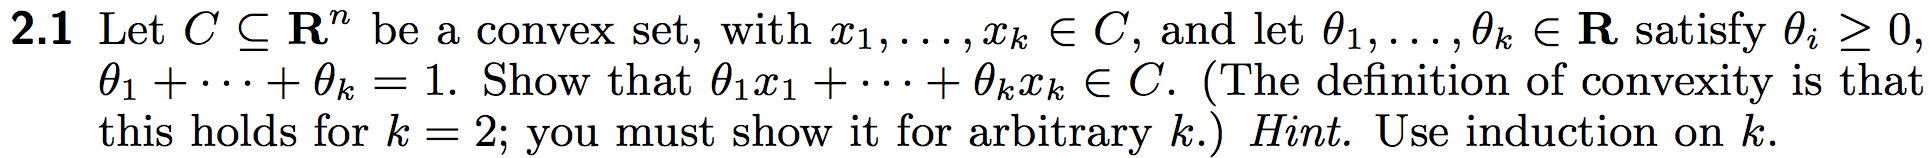
\includegraphics[width=\textwidth]{images/2-1.png}
%     \end{figure}
% \end{homeworkProblem}

\begin{homeworkProblem}
    Textbook Exercises 3.2
    \\

    \solution

    According to these curves, we can get:
    \begin{enumerate}
        \item these sublevel sets are convex \(\Longrightarrow f\) could be convex
        \item these superlevel sets are not convex \(\Longrightarrow f\) is not concave or quasiconcave
    \end{enumerate}

    \begin{figure}[h]
        \centering
        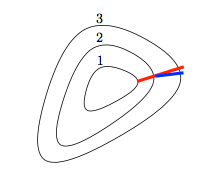
\includegraphics[width=0.3\textwidth]{images/3-2.png}
        \caption{}
        \label{3-2:1}
    \end{figure}

    As figure \ref{3-2:1} shows, take two points at \(f(x) = 1\) \(f(x) = 2\) and draw a line. From \(f(x) = 2\) to \(f(x) = 3\), the relative below line is shorter. Thus, \(f\) is not convex.

    For second level sets, we can see that the superlevel sets are convex but sublevel sets are not convex. Thus \(f\) could be concave and quasiconcave but could not convex.

\end{homeworkProblem}

\pagebreak

\begin{homeworkProblem}
    Textbook exercise 3.3
    \\

    \solution

    From \(g(f(x) = x\) we can get
    \[
        g'(f(x)) = 1/f'(x), g''(f(x)) = - \frac{f''(x)}{f'(x)^{3}}
    \]
    In addition, \(\mathbf{dom} g\) is convex. Thus g is concave.


\end{homeworkProblem}

\pagebreak

\begin{homeworkProblem}
    Textbook exercise 3.16
    \\

    \solution

    (a)
    \begin{itemize}
        \item \(e^{x}\) is convex. So \(f(x)\) is convex
        \item and therefore it is quasiconvex.
        \item \(-f(x)=1-e^{x}\) is not convex. Thus \(f\) is not concave.
        \item it is also qusiconcave because all of its super level sets are convex.

    \end{itemize}

    (b)
      \begin{itemize}
        \item The Hessian of f is
        \[
            \nabla^{2}f(x) = \left[\begin{array}{ll} 0 & 1 \\ 1 & 0 \end{array}\right]
        \]
        Thus f is not convex or concave.
        \item its superlevel sets \(\{(x_{1},x_{2}) \in \mathbf{dom} f | x_{1}x_{2} \geq \alpha\}, \forall \alpha \in \mathbb{R}^{2}_{++} \) are convex. Thus \(f\) is quasiconcave.
        \item its sublevel sets are not convex. Thus \(f\) is not quasiconvex.


    \end{itemize}

    (c)
    \begin{itemize}
        \item The Hessian of \(f\) is
        \[
            \nabla^{2}f(x) = \frac{1}{x_{1}x_{2}}\left[ \begin{array}{cc}2/x_{1}^{2} & 1/x_{1}x_{2} \\ 1/x_{1}x_{2} & 2/x_{2}^{2}\end{array}\right]
        \]
        where \(x_{1},x_{2} \in \mathbb{R_{++}}\). Thus \(\nabla^{2}f(x) \succeq 0\) and \(f\) is convex and quasiconvex.
        \item its superlevel sets are not convex. Thus \(f\) is not quasiconcave.
        \item \(-f\) is not convex. Thus \(f\) is not concave.
    \end{itemize}

    (d)
    \begin{itemize}
        \item The Hessian of \(f\) is
        \[
            \nabla^{2}f(x) = \left[ \begin{array}{cc}0 & -1/x_{2}^{2} \\ -1/x_{2}^{2} & 2x_{1}/x_{2}^{3}\end{array}\right]
        \]
        which is not positive semidefinite or negative semidefinite. Thus \(f\) is not convex or concave.

        \item its superlevel sets and sublevel sets are \(\{(x_{1},x_{2}) \in \mathbf{dom} f | x_{1}/x_{2} \geq \alpha \}\) and \(\{(x_{1},x_{2}) \in \mathbf{dom} f | x_{1}/x_{2} \leq \alpha \}\). Both are halfspaces and therefore convex. Thus \(f\) is quasiconvex and quasiconcave.
    \end{itemize}

    (e)
    \begin{itemize}
        \item The Hessian of \(f\) is
        \[
            \nabla^{2}f(x) = \left[ \begin{array}{cc} 2/x_{2} & -2x_{1}/x_{2}^{2} \\ -2x_{1}/x_{2}^{2} & 2x_{1}^{2}/x_{2}^{3} \end{array}\right] \succeq 0.
        \]
        Thus \(f\) is convex and quasiconvex.
        \item obviously \(-f\) is not convex and its superlevels sets are not convex. Thus \(f\) is not concave or quasiconcave.
    \end{itemize}

    (f)
    \begin{itemize}
        \item The Hessian of \(f\) is
        \[
            \nabla^{2}f(x) = \left[ \begin{array}{cc}
            \alpha\left(\alpha-1\right)x_{1}^{\alpha-2}x_{2}^{1-\alpha} & \alpha\left(1-\alpha\right)x_{1}^{1-\alpha}x_{2}^{-\alpha}
            \\
            \alpha\left(1-\alpha\right)x_{1}^{1-\alpha}x_{2}^{-\alpha} & -\alpha \left(1-\alpha\right)x_{1}^{\alpha}x_{2}^{-\alpha-1}
            \end{array}
            \right] \preceq 0
        \]
        Thus \(f\) is concave and quasiconcave.
        \item \(f\) is not convex or quasiconvex.
    \end{itemize}

\end{homeworkProblem}
\pagebreak

\begin{homeworkProblem}
    Textbook exercise 3.24 a-f
    \\

    \solution

    (a)
    \[\mathbf{E}(x) = \sum_{x=a_{i}}^{a_{n}} xp_{i} = \sum_{i=1}^{n} a_{i}p_{i}\]
     is a affine function and therefore it is convex, quasiconvex, concave, and quasiconcave.
    \\

    (b)
    \[\mathbf{prob}(x \geq \alpha)  = \sum_{i=j}^{n}a_{i}p_{i},
    \]
    where
    \[a_{j} = min\{a_{i} \geq \alpha | i=1,2,\dots,n\}\]
    Similar to (a), it is also convex, quasiconvex, concave and quasiconcave.
    \\

    (c)\[
    \mathbf{prob}(\alpha \leq x \leq \beta)  = \sum_{i=j}^{k}a_{i}p_{i}\]where \[a_{j} = min\{a_{i} \geq \alpha | i=1,2,\dots,n\}, a_{k} = max\{a_{i} \leq \beta | i=1,2,\dots,n\}\]
    Similar to (a)(b), it is also convex, quasiconvex, concae, and quasiconcave.
    \\

    (d)
    \(\sum_{i=1}^{n}p_{i}\log p_{i}\) is convex and quasiconvex because negative entropy is convex and quasiconvex. And its superlevel sets are not convex. Thus it is not quasiconcave or concave.
    \\

    (e)
    \[
        var(x) = \sum_{i=1}^{n} a_{i}^{2}p_{i} + \left(\sum_{i=1}^{n}a_{i}p_{i}\right)^{2}
    \]
    is a quadratic function of p and therefore it's concave and quasiconcave.
    \\

    (f)Its superlevel sets and sublevel sets are convex. Thus \(\mathbf{quartile}(x)\) is quasiconvex and quasiconcave. And it is not continuous and therefore it is not convex or concave.
    \\

\end{homeworkProblem}



\end{document}
